\documentclass[custom]{sciposter}
\usepackage{graphicx}
\usepackage{multicol}
\institute{Western Pacific Tropical Research Center, University of Guam, Mangilao, Guam  96923, USA }
\leftlogo[0.6]{gv/images/uoglogo.png}
\rightlogo[0.7]{gv/images/calslogo.png}
\title{A Coalition of Invasive Species\\Attacks Guam's Endemic Cycad, \textit{Cycas micronesica}}
\author{Aubrey Moore, Ross H. Miller, Thomas E. Marler and Lee S. Yudin}
\renewcommand{\titlesize}{\Huge}

% Reduce top and bottom margins
\addtolength{\topmargin} {-1in}
\addtolength{\textheight} {2in}

% Reduce left and right margins
\addtolength{\oddsidemargin}{-1in}
\addtolength{\evensidemargin}{-.1in}
\addtolength{\textwidth}{2in}

\begin{document}
\maketitle

\begin{figure}
\centering
%\frame{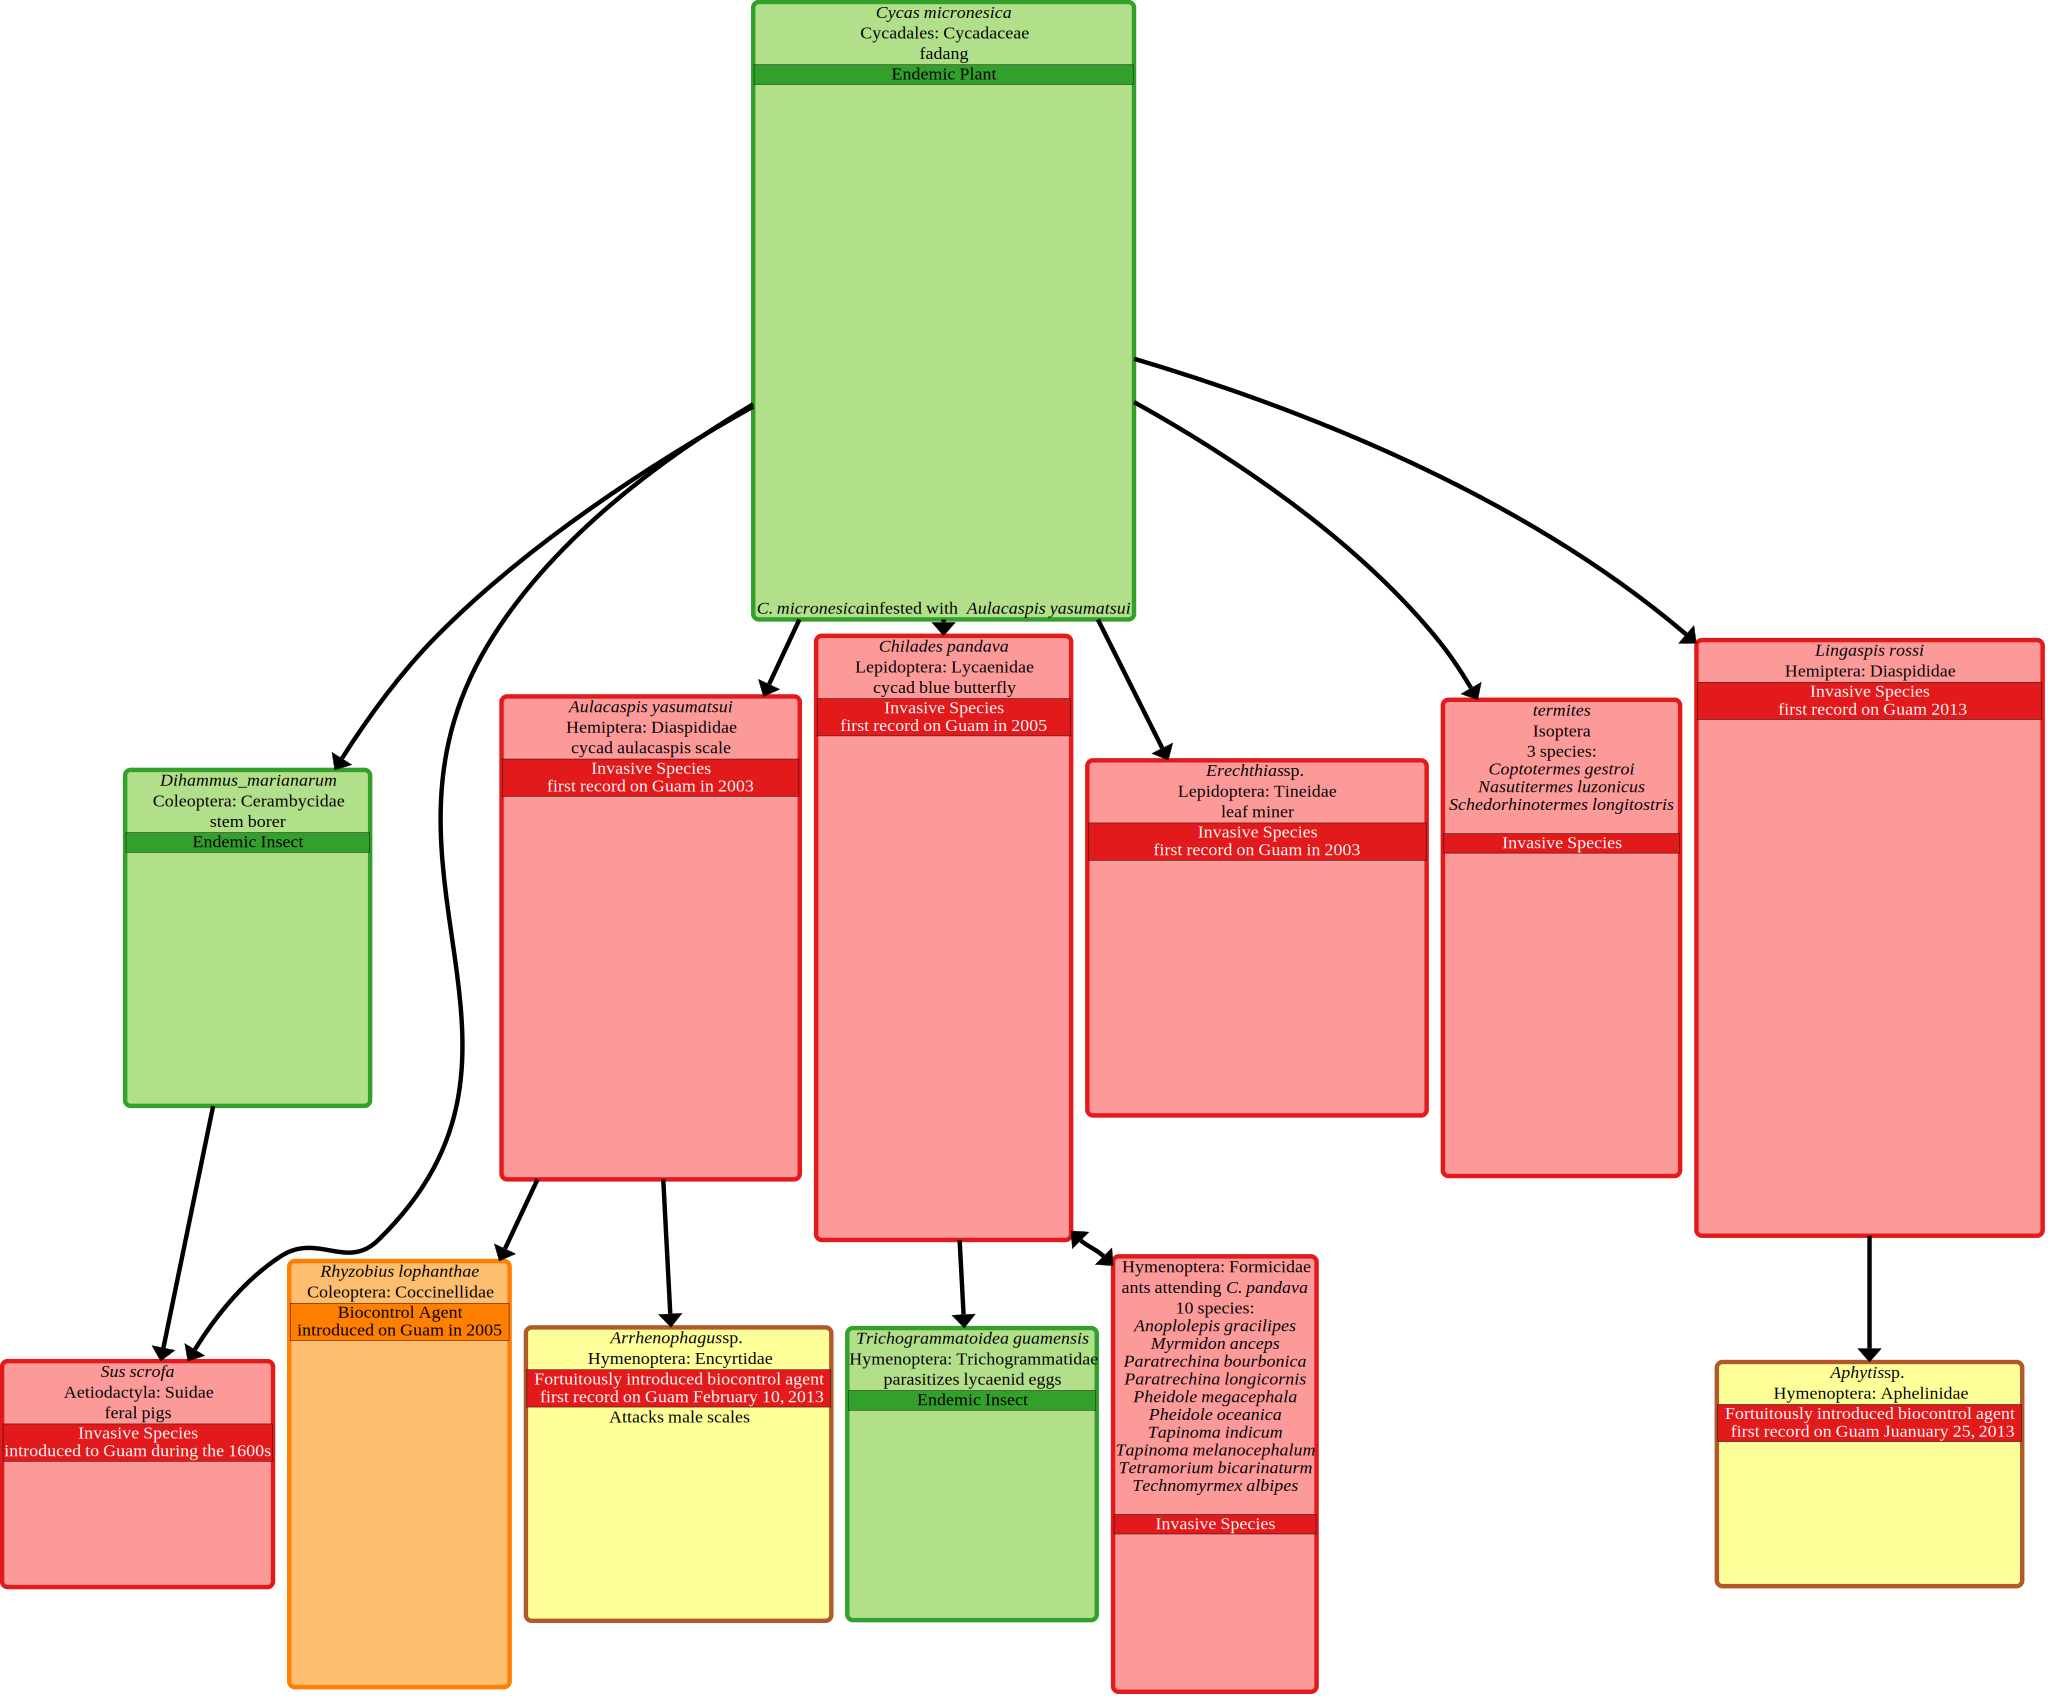
\includegraphics[height=0.65\textheight]{gv/graph1.pdf}}
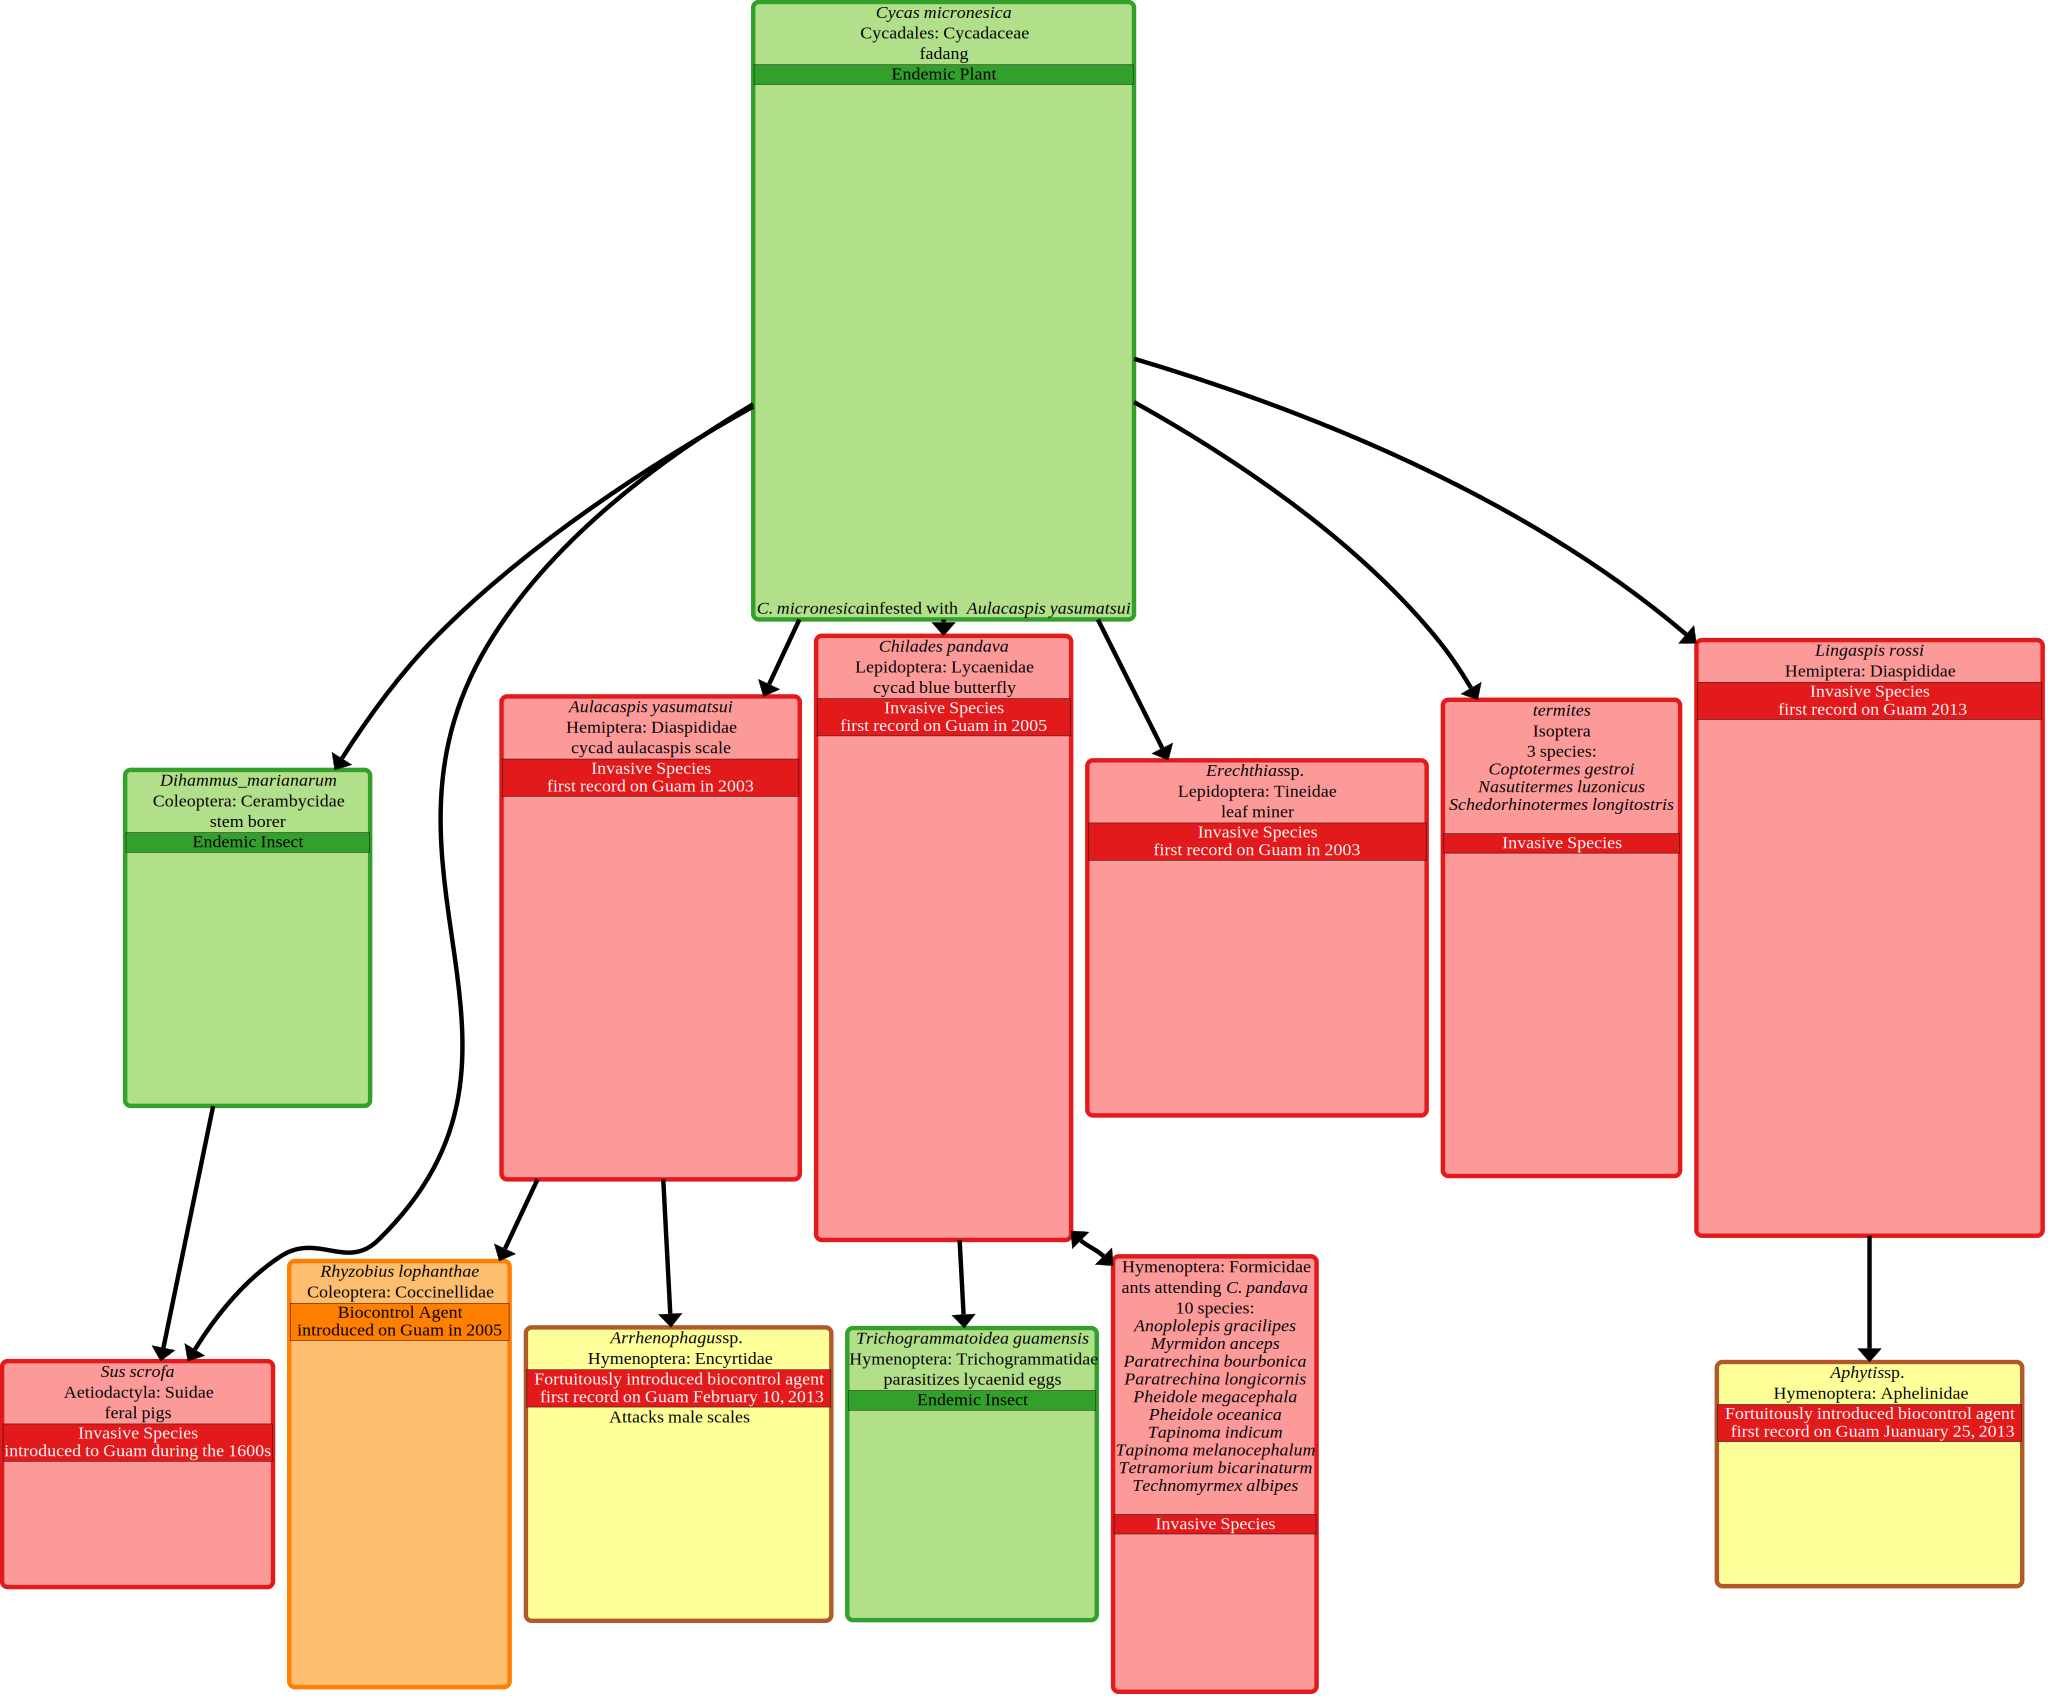
\includegraphics[height=0.60\textheight]{gv/graph1.pdf}
\caption{\textnormal{Summary of ecological relationships between} \textit{C. micronesica} \textnormal{and invasive species which threaten its existence. Arrows indicate which species benefit from relationships.}}
\end{figure}

% Overlay legend using \put(x,y) for absolute positioning
\begin{picture}(50,50) 
  \put(1570,1150){\hbox{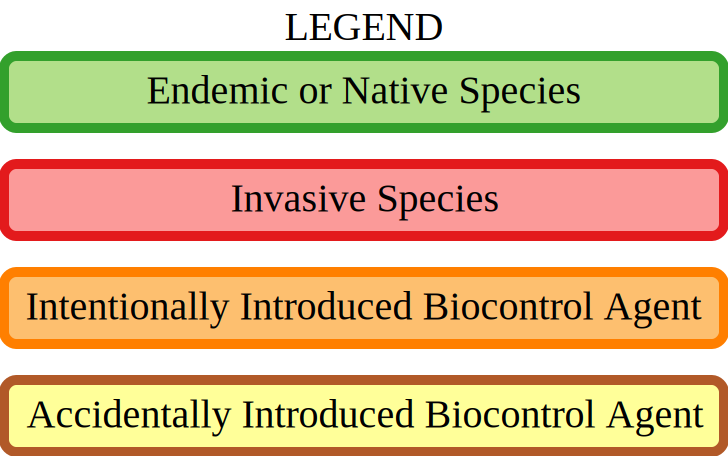
\includegraphics{gv/legend.pdf}}}
\end{picture}
  
\begin{multicols*}{3}
A 2002 forest survey listed \textit{Cycas micronesica}, locally known as "fadang", as the most numerous tree-sized plant in Guam's forests.   In 2006 \textit{C. micronesica} was placed on the IUCN Red List of Threatened Species in response to high mortality from simultaneous attack by recently introduced invasive species including the cycad aulacaspis scale (CAS), \textit{Aulacaspis yasumatsui}, the cycad blue butterfly, \textit{Chilades pandava}, and a lepidopteran leafminer, \textit{Erechthias} sp.  The coccinellid, \textit{Rhyzobius lophanthae} was established as an effective biological control agent for CAS.  However, the cycads continue to decline due to damage from CAS and other herbivores.  In some areas of Guam, 90\% of \textit{C. micronesica} have been killed and the plant could be extirpated from the wild by 2019 if current trends persist.
\columnbreak
\section*{References}

\textbf{Moore, A., T. Marler, R.H. Miller and R. Muniappan. 2005.} Biological control of cycad aulacaspis scale on Guam. The Cycad Newsletter 28(5):6-8. 
\newline
\textbf{Marler, T.E. and R. Muniappan.  2006.}  Pests of \textit{Cycas micronesica} leaf, stem, and male reproductive tissues with notes on current threat status.  Micronesica 39: 1-9.
\newline
\textbf{Marler, T. E. and A. Moore 2010.} Cryptic scale infestations on \textit{Cycas revoluta} facilitate scale invasions. HortScience 45(5): 837–839.
\newline
\textbf{Marler, T. E., L. S. Yudin and A. Moore 2011.} \textit{Schedorhinotermes longirostris} (Isoptera: Rhinotermitidae) on Guam adds to assault on the endemic \textit{Cycas micronesica}. Florida Entomologist 94(3): 702-703.
\newline
\textbf{Marler, T.E. and J.H. Lawrence 2012.} Demography of \textit{Cycas micronesica} on Guam following introduction of the armoured scale \textit{Aulacaspis yasumatsui}. J. Trop. Ecol. 28:233–242.
\newline
\textbf{Marler, T. E. 2013.} Temporal variations in leaf miner, butterfly, and stem borer infestations of \textit{Cycas micronesica} in relation to
\textit{Aulacaspis yasumatsui} incidence. HortScience 48(10):1334–1338. 
\newline
\textbf{Marler, T. E. \& J. H. Lawrence 2013.} Phytophagous insects reduce cycad resistance to tropical cyclone winds and impair storm recovery. HortScience 48(10):1224–1226.

\section*{ACKNOWLEDGMENTS}

Data are from projects supported by grants from the US Forest Service, the US Fish and Wildlife Service, and USDA-APHIS.

\end{multicols*}
\end{document}